\chapter[Theory]{Theory}
The following chapter gives an introduction to the theory behind this work. Some of the sections only give a brief description of the theory with sources for more in depth explanation. %The main focus of this chapter is describing the theory behind the Markov chain Mote Carlo method for solving extreme value problem developed for this paper. 
\section{Extreme value theory}
%The basics of extreme value theory is to analyze
The basics of extreme value theory, is to analyze the maximum of a series of random variables $X_1,\dots,X_n$.
Defining $M_n$ as the maximum of a series
\begin{equation}
M_n=\max\{X_1,\dots,X_n\},
\end{equation}
%
the resulting distribution of $M_n$ is
\begin{equation}
\label{eq:basicextreem}
\Pr(M_n \leq z)=\Pr(X_1 \leq z,\dots, X_n \leq z).
\end{equation}
By assuming $X_1,\dots,X_n$ independent and identically distributed (i.i.d.) with common cumulative distribution function $F$, equation \eqref{eq:basicextreem} reduces to
\begin{align}
\begin{split}
    \Pr(M_n \leq z)&=\Pr(X_1 \leq z)\times \dots \times \Pr(X_n \leq z)\\
    &=\big[F(z)\big]^n.   
\end{split}
\end{align}
The distributing $F$ is normally unknown, and a divergent in the estimated distributing $F$ could potentially escalate to a large difference in the resulting $F^n$. 

As for the central limit theory for the normal distribution, $F^n$ also has a limiting distribution, by The Fisher–Tippett–Gnedenko theorem. If there exist an $a_n>0$ and $b_n$ such that 
\begin{equation}
\lim_{n \to \infty} \Pr\big[(M_n-b_n)/a_n \leq z\big]\to G(z),
\end{equation}
where $G$ is a non-degenerating function, then $G$ follows either
%\begin{align}
%G(z) &=\exp\Big\{-\exp\Big[-\Big( \frac{z-b}{a}\Big) \Big]\Big\}, & \quad -\infty < z < \infty;\label{eq:gumbel}\\
%G(z) &=
%  \begin{cases}
%    0, & \quad z\leq b,\\
%    \exp\big\{-\big(\frac{z-b}{a} \big)^{-\alpha} \big\},  & \quad z>b;\\
%  \end{cases} \label{eq:frechet}\\
%G(z) &=
%  \begin{cases}
%    \exp\Big\{-\Big[-\Big( \frac{z-b}{a}\Big) \Big]^{\alpha}\Big\}, & \quad z\leq b,\\
%    1,  & \quad z>b;\\
%  \end{cases} \label{eq:weibull}\\
%\end{align}

\begin{align}
G(z) &=\exp\Big\{-\exp\Big[-\Big( \frac{z-b}{a}\Big) \Big]\Big\},  & -\infty < z < \infty;\label{eq:gumbel}\\
G(z) &=
  \begin{cases}
    0,\\
    \exp\big\{-\big(\frac{z-b}{a} \big)^{-\alpha} \big\},  
  \end{cases}
 \begin{split}
   &z\leq b, \\
   &z >b;\label{eq:frechet}\\
  \end{split}\\
G(z) &=
  \begin{cases}
    \exp\Big\{-\Big[-\Big( \frac{z-b}{a}\Big) \Big]^{\alpha}\Big\}, \\
    1,  
  \end{cases}  
 \begin{split}
   &z \leq b,\\
   &z>b;\label{eq:weibull}
  \end{split}
\end{align}
for each case, $\alpha>0$. Here equation \eqref{eq:gumbel}, \eqref{eq:frechet} and \eqref{eq:weibull} refears to Gumbel, Fr{\'e}chet and Weibull distribution respectively. The above equation can be combined into the General Extreme Value (GEV) distribution
\begin{equation}
\label{eq:GEV}
G(z)=\exp\Bigg\{-\Big[1+\xi \Big(\frac{z-\mu}{\sigma} \Big) \Big]^{-\frac{1}{\xi}} \Bigg\}
\end{equation}
where $1+\xi(z-\mu)/\sigma>0$, the location parameter is $-\infty<\mu<\infty$, the scale parameter is $\sigma>0$ and the shape parameter is $-\infty<\xi<\infty$. It can easily be verified that the GEV equals equation \eqref{eq:frechet} when $\xi>0$, equation\eqref{eq:weibull} when $\xi<0$ and converge towards equation\eqref{eq:gumbel} as $z \to 0$.

The GEV model requires i.i.d. data points for parameter estimations. Unfortunately, in practice that is rarely the case. Block maxima or r largest order statistics are common methods for filtering the dependent data points into an approximate i.i.d. dataset \cite[p.~66]{stuart}. The basic principle is to only use the largest, or r largest data within each block. Examples of block sizes could be week, month, year etc.

For a deeper description of extreme value theory, GEV or block maxima, the book of \cite[Chapter~3]{stuart} is suggested.

\subsection{Peak Over Threshold} 
One of the problem with the GEV method and the i.i.d. filtration of data points, is that the block maxima and r largest order statistics are quite wasteful. Specially in situations where some blocks contains more extreme than others, large extreme will be discarded from the set, which else would have been accepted in other blocks.

The Peak Over Threshold (POT) method is suggesting a different method of tackling the i.i.d. filtration. Filtering the data, by only using points over a certain threshold $u$, avoid the problem of discarding large extremes in certain blocks. As long as $u$ is chosen sufficiently large, the resulting data will be i.i.d. Using the GEV distribution equation \eqref{eq:GEV} it can be shown, like was done by \cite[p.~76]{stuart}, that 
\begin{equation}
\label{eq:potCond}
\Pr(X>y+u|X>u)=\Big(1+\frac{\xi y}{\tilde{\sigma}}\Big)^{-\frac{1}{\xi}},
\end{equation}
where $y$ is the threshold excess, given by $y=z-u$ for $z>u$.
The resulting distribution of $y$ is called the generalized Pareto distribution (GPD)
\begin{equation}
\label{eq:potwxi}
H(y)=1-\Big(1+\frac{\xi y}{\tilde{\sigma}}\Big)^{-\frac{1}{\xi}}
\end{equation}  
or
\begin{equation}
\label{eq:potwoxi}
H(y)=1-\exp\Big(-\frac{y}{\tilde{\sigma}}\Big)
\end{equation}
when $\xi \to 0$. Here $\xi$ equals the GEV parameter, while $\tilde{\sigma}=\sigma+\xi(u-\mu)$.
The conditional probability
\begin{align}
\Pr(X>y+u|X>u)& = \frac{\Pr(X>y+u,X>u)}{\Pr(X>u)} \nonumber\\
&=\frac{\Pr(X>y+u)}{\Pr(X>u)}, \label{eq:potPredBetween} 
\end{align}

since $y+u \geq u$, the probability $\Pr(X>y+u, X>u)=\Pr(X>y+u)$.
By combining equation \eqref{eq:potCond} and \eqref{eq:potPredBetween}, the probability of a future event can be found by
\begin{align}
\Pr(X>z)&=\Pr(X>y+u) \nonumber\\
 		&=\Pr(X>u) \cdot P(X>y+u|X>u)\nonumber\\
 		&=\Pr(X>u) \cdot \left[1+\xi \left( \frac{z-u}{\tilde{\sigma}}\right)\right]^{-\frac{1}{\xi}}, \label{eq:potPred}
\end{align}
where $\Pr(X>u)$ is the probability that a random point exceeds the threshold.

For more information about the POT method, see \cite[Chapter~4]{stuart}.\\
\\
\textcolor{red}{ADD/TALK/NAME GENERALIZED PARETO DISTRIBUTION (GPD) (H(y)).\\
y=x-u CALLED THRESHOLD EXCESS. INCLUDE IN OTHER PARTS OF THE THESIS!}


\subsubsection{Declustering}
The numbers of threshold excess $y$ increase as the threshold $u$ decrease. A larger number of threshold excess will increase the accuracy and lower the variance of the parameter estimation, which suggest using a low threshold. In practice, data are often correlated, heteroscedastic or nonstationary. For data without trend, a high enough threshold will ensure close to  i.i.d. property for the threshold excess. As the threshold decrease, clusters could appear, and the threshold excess will no longer be i.i.d. Violation of the i.i.d. property will result in an estimation bias, which suggest using a high threshold. The selection of threshold comes down to the trade-off between accuracy and bias. The goal is to get the lowest variance without bias.

Declustering method can be applied to improve the i.i.d. property for low threshold. The target is to localize clusters above the threshold and select the largest value within each cluster. The method used here, defines a cluster as the points above the threshold, until $r$ consecutive points are observed below. Referring to figure \ref{fig:declustplot}, for an example on how the method is used in practice. For $r=1$ there are 7 clusters, while for $r=4$ there are 3. For the particular threshold used in the plot, $r=4$ seems like the superior choice. 

For a more in depth description of decluttering, see \cite[p.~100]{stuart}.
\begin{figure}
  \centering
    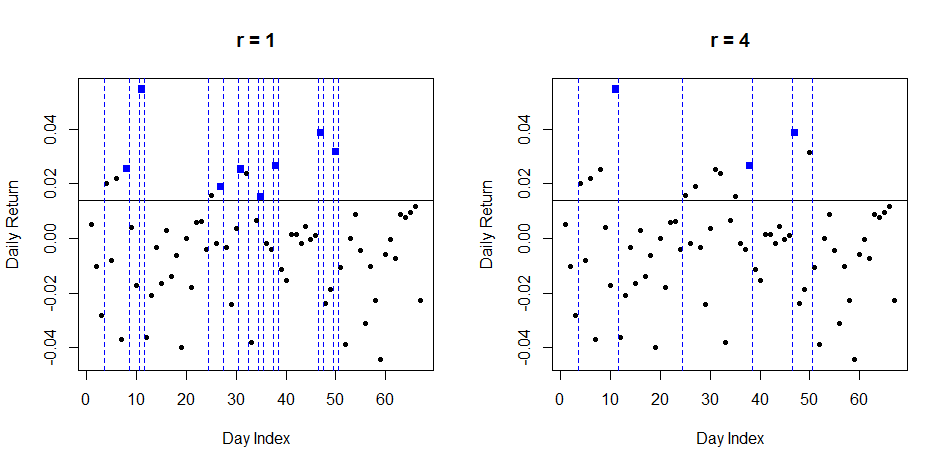
\includegraphics[width=1\textwidth]{fig/declustplot.png}
  \caption{Portion of the crude oil daily return series, described in chapter \ref{ch:comdata}. The horizontal solid line is threshold, with $u=0.014$. Clusters are localized between the vertical blue dashed lines, with the largest value within each clusters shown as a blue square.}
  \label{fig:declustplot}
\end{figure}

\subsubsection{Threshold}
As stated above, the goal when selecting threshold $u$ is to find the smallest threshold $u_0$, for which the model is still unbiased, such that the highest accuracy is achieved. For this paper, the combination of two methods are used in the selection process. 

The first method uses the fact that the mean of the GPD equals 
\begin{equation}
E(Y)=\frac{\tilde{\sigma}}{1-\xi}, 
\end{equation}
for $\xi<1$, and infinite when $\xi>1$. Thus the first method fails when $\xi>1$, but in practice $\xi$ rarely exceeds $1$.
As shown above, the GPD $\xi$ equals the GEV parameter which is independent of threshold, while $\tilde{\sigma}=\sigma+\xi (u-\mu)$ is linear with respect to threshold. Here $\sigma$ and $\mu$ are the GEV parameters and independent of threshold.
Thereby the mean of $Y$ is also linear proportional to threshold. By plotting the mean of threshold excess against thresholds, linear effect should be apparent from $u_0$. Confidence interval can be added for a better understanding of where the linearity starts. For larger values of thresholds, there will only be a few numbers of threshold excess, hence it is suggested using t-distribution for more realistic confidence intervals. \textcolor{red}{REFERING TO PLOT BLABLABLA}. For more information about the method, see \cite[p.~79]{stuart}.

For the second method, estimates of $\xi$ and $\tilde{\sigma}$ is taken for a variety of thresholds. The parameters $\xi$ and the reparametrized $\sigma \mbox{*}=\tilde{\sigma}-\xi u$ should both be constant from $u_0$. For pinpointing of $u_0$, both $\xi$ and $\sigma \mbox{*}$ is plotted against $u$, with added confidence intervals.  \textcolor{red}{REFERING TO PLOT BLABLABLA}. For more information about the method, see \cite[p.~83]{stuart}.

After threshold selection, $\tilde{\sigma}$ is simply estimated from the threshold excess and is required larger than zero. For simplicity, from here, the notation $\sigma$ is used for the GPD parameter $\tilde{\sigma}$, as long as otherwise is not specified. 

\subsection{Average Condition Exceedance Rate}
The Average Conditional Exceedance Rate (ACER) is another extreme value method, first introduced by \cite{arvid0}, see the paper and \cite{arvid} for a more in depth description of the theory, as the following is only a brief introduction. 
Both the GEV and GPD distributions requires the observations to be i.i.d. When observations are not i.i.d., filtering methods such as, threshold exceedance, declustering, blocking, etc., is used to achieve close to i.i.d. data. The problem with these filtering methods, is that they often discard most of the data, such that only a small amount of the data can be used for parameter estimation. The advantage of the ACER method is that the observation is not restricted to i.i.d. or even stationarity data, only requires no trend. Another advantage is the ACER methods ability to a certain extent capture the subasymtotic parts, which also could improve estimation.

Without the i.i.d. assumption for $X_1,\dots,X_n$, equation \eqref{eq:basicextreem} can be written using time dependency
\begin{equation}
\label{eq:extreemdepend}
\Pr(M_n \leq z)=\prod_{j=1}^{n} \Pr(X_j \leq z,| X_{j-1} \leq z,\dots, X_1 \leq z)\cdot \Pr(X_1 \leq z).
\end{equation}
It is reasonable to assume that the data dependency with neighboring points degrease by time, and is negligible after $k \ll n$ steps, such that \\${\Pr(X_j \leq z,| X_{j-1} \leq z,\dots, X_1 \leq z) \approx \Pr(X_j \leq z,| X_{j-1} \leq z,\dots, X_{j-k+1} \leq z) }$ for every $j=k,\dots, n$. Using this and tailor expansion of the exponential function around zero, equation \eqref{eq:extreemdepend} reduces to
\begin{align}
\Pr(M_n \leq z)&\approx \exp\left( -\sum_{j=k}^{n} \alpha_{kj}(z) -\sum_{i=1}^{k-1} \alpha_{ii}(z) \right) \nonumber\\
			&\approx \exp\left( -\sum_{j=k}^{n} \alpha_{kj}(z) \right)
\end{align}
where $\alpha_{kj}(z)=\Pr(X_j \geq z |X_{j-1} \leq z, \dots, X_{j-k+1}\leq z)$ for $k\geq 2$ and $\alpha_{kj}(z)=\Pr(X_j \geq z)$ for $k=1$. The final step is justified since $\sum_{i=1}^{k-1} \alpha_{ii}(z)$ is negligible compared to $\sum_{j=k}^{n} \alpha_{kj}(z)$ for $k \ll n$, while the tailor expansion around zero is reasonable at the upper tail since for large $z$, $\alpha_{kj}(z)$ is close to zero.

Considering the Average Conditional Exceed Rate (ACER) as
\begin{equation}
\epsilon_k(z)=\frac{1}{n-k+1} \sum_{j=k}^{n} \alpha_{kj}(z).
\end{equation}
The ACER function can be estimated using
\begin{equation}
\label{eq:epsest}
\hat{\epsilon}_k(z)=\frac{\sum_{j=k}^n \mathbf{1}(x_{j} \geq z, x_{j-1} \leq z, \ldots, x_{j-k+1} \leq z)}{\sum_{j=k}^n \mathbf{1}(x_{j-1} \leq z, \ldots, x_{j-k+1} \leq z)}.
\end{equation}
where $\mathbf{1}(\omega)$ is the indicator function for event $\omega$. For nonstationary observations it is suggested using $n-k+1$ as an approximation for the denominator. The approximation can be justified since $ \mathbf{1}(x_{j-1} \leq z, \ldots, x_{j-k+1} \leq z) \to 1$ in the upper tail where z is large. 

It is assumed that the tail of the ACER function follows 
\begin{equation}
\label{eq:acerest}
\epsilon_{k}(z|a_k,b_k,c_k,q_k,\xi_k)=q_{k} \left[ 1+\xi_k \left( a_k (z-b_k)^{c_k} \right) \right]^{-1/\xi_k},
\end{equation}
where the parameters $a_k$, $b_k$, $c_k$, $q_k$ and $\xi_k$ are approximately constant in the upper tail for a certain $k$. The process of selecting $k$ can be done by investigating the plot of $\hat{\epsilon}_k(z)$ against $z$ for a verity of $k$, $k$ is set to the smallest value for which increasing $k$ makes negligible change to the tail. see figure \textcolor{red}{REF TIL FIGUR PLUS SOME TEXT HER!!!!!!!!!!}. 
The parameters can be estimated by minimizing the weighted square error
\begin{equation}
\label{eq:acerse}
F(a,b,c,q,\xi)=\sum_{i=1}^{N} w_i \left[ \log \left( \hat{\epsilon}_k(z_i)\right)-log(q)+\xi^{-1} \log \left( 1 + a(z_i-b)^c \right) \right]^2,
\end{equation}
using numerical methods. Selecting $z_1,\dots,z_N$ is done by uniformly dividing the values from where regular tail behavior of $\hat{\epsilon}_k(z)$ starts to $\smash{\displaystyle\max_{1 \leq i \leq n}(X_i)}$ into $N$ points. The weights $w_i$ is calculated using 
\begin{equation}
w_i=\left( \log \left[ C_{\alpha}^{+}(z_i)\right] - \log \left[ C_{\alpha}^{-}(z_i) \right] \right)^{-2},
\end{equation}
where $C_{\alpha}^{+}(z_i)$ and $C_{\alpha}^{-}(z_i)$ is the upper and lower $100 \cdot \alpha\%$ confidence interval values respectively for $\hat{\epsilon}_k(z_i)$. Organizing the observation into $R$ similar realizations, like $R$ years, the sample variance can be calculated as 
\begin{equation}
\hat{s}_k(z_i)^2=\frac{1}{R-1} \sum_{r=1}^{R} \left( \hat{\epsilon}^{(r)}_k(z_i) - \hat{\epsilon}_k(z_i) \right)
\end{equation}
where $\hat{\epsilon}^{(r)}_k(z_i)$ is the estimated ACER function for the $r$ realization at $z_i$.
Hence a $100 \cdot \alpha\%$ confidence interval can be calculated using the student t-distribution
\begin{equation}
C_{\alpha}^{\pm}(z_i)=\hat{\epsilon}_k(z_i) \pm t_{(1-\alpha)/2,R-1} \frac{\hat{s}_k(z_i)}{\sqrt{R}}
\end{equation}
where $t_{p,\nu}$ is defined as $\Pr(T>t_{p,\nu})=p$ for the standardized $t$ distribution with $\nu$ degrees of freedom.

After parameter estimation, future prediction can be achieved using equation \eqref{eq:acerest}. Confidence intervals can be added to the ACER function prediction by estimating the parameters to the upper and lower confidence curve. Using $\epsilon_{k}(z_i|a,b,c,q,\xi) \pm t_{(1-\alpha)/2,R-1} \frac{\hat{s}_k(z_i)}{\sqrt{R}}$ instead of $\hat{\epsilon}_k(z_i)$ in equation \eqref{eq:acerse}, where $\epsilon_{k}(z_i|a,b,c,q,\xi)$ is given by equation \eqref{eq:acerest}, parameters for upper and lower confidence curves are estimated. These upper and lower confidence parameters can be used in equation \eqref{eq:acerest} for ACER function prediction confidence intervals.
\\ \\
\textcolor{red}{HUSK SKRIV OM PLOT FOR ACER TIL z I STEDET FOR $\eta$!!!!!!!!!!}

\subsection{Predicting Future Extreme With Confidence Interval}
highest posterior density interval (Choosing the narrowest interval)


\section{Bayesian Inference}
\label{ch:BayesianInference}
For the traditional frequentist statistics, the parameters $\boldsymbol{\theta}$ are assumed fixed, while data $x_1,\dotsc ,x_n$ are random from the underlying distribution $f(\boldsymbol{x}| \boldsymbol{\theta})$. Bayesian statistics, instead treats the parameters $\boldsymbol{\theta}$ with a probability distribution, where it is possible to make subjective believes about the distribution, independent of the data. These subjective beliefs is used to construct a prior distribution $f(\boldsymbol{\theta})$ based on experiences, information or physical knowledge of the situation analyzed. 

The posterior distribution of the parameters dependent on the measured data becomes 
\begin{equation}
f(\boldsymbol{\theta}|\boldsymbol{x})=\frac{f(\boldsymbol{\theta})f(\boldsymbol{x}|\boldsymbol{\theta})}{\int_{\Theta} f(\boldsymbol{\theta})f(\boldsymbol{x}|\boldsymbol{\theta}) \mathrm{d} \theta}, 
\end{equation}
where $\Theta$ is the domain over all possible parameters, for which the integral is taken, and  $f(\boldsymbol{x}|\boldsymbol{\theta})$ is the likelihood function. The likelihood function is constructed from the joint density function, which for independent data equals
\begin{equation}
\label{eq:jointdens}
f(\boldsymbol{x}|\boldsymbol{\theta})=\prod_{i=1}^{n} f(x_i|\boldsymbol{\theta}).
\end{equation}
The integral over parameters reduces to a constant, which makes
\begin{equation}
f(\boldsymbol{\theta}|\boldsymbol{x}) \sim c \cdot f(\boldsymbol{\theta})f(\boldsymbol{x}|\boldsymbol{\theta}), \label{eq:genposteriorc}
\end{equation}
where $c=1/ \int_{\Theta} f(\boldsymbol{\theta})f(\boldsymbol{x}|\boldsymbol{\theta}) \mathrm{d} \theta$ is the normalizing constant.

A conjugate prior is a prior which combined with the likelihood function construct a posterior distribution in the same family as the prior.  Conjugate priors are often preferred because of the analytical luxury and computational simplicity.\\

Since Bayesian inference accounts for the distribution of parameters, equation \eqref{eq:potPred} can be rewritten using $\Pr(X>u)=\alpha$
\begin{equation}
\Pr(X>z)=\alpha \left[1+\xi \left( \frac{z-u}{\sigma}\right)\right]^{-\frac{1}{\xi}},
\end{equation}
where $\alpha$, $\xi$ and $\sigma$ are the unknown parameters. Since $\alpha$ is the probability of a point being larger than the threshold, $\alpha$ is independent of $\xi$ and $\sigma$. For the independent parameters, development of the posterior distributions can be treated separately. 

Starting with $\xi$ and $\sigma$, by combining equation \eqref{eq:jointdens} and \eqref{eq:potwxi}, the joint density function for the POT method becomes
\begin{align}
f(\boldsymbol{y}|\xi,\sigma)&=\prod_{i=1}^{n} h(y_i|\xi,\sigma)\nonumber\\
&=\sigma^{-n} \prod_{i=1}^{n}\left( 1+\frac{\xi y_i}{\sigma}\right)^{-\left(1+\frac{1}{\xi}\right)}, \label{eq:jointdenspot}
\end{align}
or by \eqref{eq:potwoxi} for $\xi=0$, $f(\boldsymbol{y}|\sigma)=\sigma^{-n}\exp\left\{-\sigma^{-1} \sum_{i=1}^{n}y_i \right\}$.  here $h$ is the probability density function of the GPD, while $n$ is the numbers of threshold excess.

The obvious beginning for investigating priors is the conjugate priors, but unfortunately, there do not appear to be any conjugate priors for the joint GPD. This work, will not go into depth on how to select Bayesian priors for the GPD, but instead use the suggestion proposed by \cite[p.~174]{stuart}. Note that there are potential improvements by deeper investigation of GPD or GEV priors, especially for priors developed for specific situations where there are physical knowledge or practical experiences about the parameters. Since $\sigma>0$, the transformation $\phi=\log(\sigma)$ ensures $\sigma$ to be valid without restriction on $\phi$. The suggested priors are $f_{\phi}(\cdot)$ and $f_{\xi}(\cdot)$ to be normally distributed around zero with variance $v_{\phi}=10^4$ and $v_{\xi}=100$. 

Considering the prior distribution of $\phi$ instead of $\sigma$, the change of variable for the joint density function becomes 
\begin{align}
f_{\boldsymbol{y}|\xi,\phi}(\boldsymbol{y}|\xi,\phi)&=\frac{f_{\boldsymbol{y},\xi,\phi}(\boldsymbol{y},\xi,\phi)}{f_{\xi,\phi}(\xi,\phi)}\nonumber\\
&=\frac{f_{\boldsymbol{y},\xi,\sigma}\left(\boldsymbol{y},\xi,\exp(\phi)\right)\cdot \left|\frac{\mathrm d}{\mathrm d \phi} \exp(\phi)\right|}{f_{\xi,\sigma}\left(\xi,\exp(\phi)\right)\cdot \left|\frac{\mathrm d}{\mathrm d \phi} \exp(\phi)\right|}\nonumber\\
&=f_{\boldsymbol{y}|\xi,\sigma}\left(\boldsymbol{y}|\xi,\exp(\phi)\right), \label{eq:jointdenschang}
\end{align}
where $f_{X}(\cdot)$ indicates the probability distribution of $X$.
The posterior distribution of the parameters can then be developed by the priors, \eqref{eq:jointdenschang} and \eqref{eq:genposteriorc}
\begin{align}
f_{\xi,\phi|\boldsymbol{y}}(\xi,\phi|\boldsymbol{y})\sim c \cdot f_{\boldsymbol{y}|\xi,\sigma}\left(\boldsymbol{y}|\xi,\exp(\phi)\right)f_{\xi}(\xi)f_{\phi}(\phi), \label{eq:potpost}
\end{align}
where again c is the normalizing constant, $f_{\boldsymbol{y}|\xi,\sigma}$ is as in \eqref{eq:jointdenspot}, $f_{\xi}(\xi)\sim N(0,100)$ and $f_{\phi}(\phi) \sim N(0,10^4)$.

The development of $\alpha$ posterior distribution, can be started with investigating priors. Since $\alpha$ simply equals $\Pr(X>u)$, the range is limited between $0$ and $1$. For simplicity the prior is set proportional to the uniform distribution on the interval $(0,1)$, $f(\alpha) \sim UNIF(0,1)$. It is noted that in reality the distribution of $\alpha$ is not flat. Low valued $\alpha$ is more probably then high, while the probability converges to zero for the endpoints. A well-tuned Beta distributed prior could account for this, and improve the result.

The joint density function can be created by the fact that $\alpha$ simply equals the probability of a random point exceeding the threshold. This can be expressed using the binominal distribution, $k_i$ for the numbers of points exceeding the threshold and $N_i$ for the total numbers of point, each for a given period $i$. For a total $m$ numbers of periods, the posterior distribution equals
\begin{align}
f(\alpha|k_1,\dotsc,k_n, N_1, \dotsc, N_n)&\sim f(\alpha)\cdot \prod_{i=1}^{m} f(k_i|N_i,\alpha)\nonumber\\
&=\prod_{i=1}^{m} \binom{N_i}{k_i} \alpha^{k_i}(1-\alpha)^{N_i-k_i}\nonumber\\
& \sim \alpha^{\sum_{i=1}^{m}k_i}(1-\alpha)^{\sum_{i=1}^{m}N_i-\sum_{i=1}^{m}k_i}.\label{eq:alphaposttemp}
\end{align}
The resulting distribution is independent of period selection, the notation $k$ and $N$ can be used for the total numbers of exceedance and the total numbers of measurements respectively. It is noted that the distribution is proportional to the Beta distribution. Since there only exist one normalizing constant which fulfills the requirements for a probability distribution, the posterior distribution is not only proportional, but equal to the Beta distribution. Rewriting equation \eqref{eq:alphaposttemp} gives
\begin{equation}
\label{eq:alphapost}
f(\alpha|k,N) \sim BETA(k+1,N-k+1).
\end{equation}

\section{Markov Chain Monte Carlo Method}
\label{ch:mcmc}
%High dimentional problem (TMA4300 2014 first mcmc)
Markov Chain Monte Carlo (MCMC) is a powerful iterative method used to sample from probability distributions, which analytically or through other simulation methods, could be difficult and impracticable to sample from. The algorithm is constructed by converging the desired probability distribution to an irreducible and aperiodic Markov Chain with limiting distribution equal the target distribution. Independent of starting position the Markov Chain will then converge towards the desired probability distribution in the limit as the numbers of iterations goes to infinity. The first numbers of realizations from the Markov Chain until converging is called the burn-in period, and is discarded for further analyses. More information about burn-in can be found in \cite[p.220]{compstat}. The remaining realizations, approximately follows the desired probability distribution, where the accuracy increase as the numbers of realizations increase. Monte Carlo method can then be used to calculate the quantity of interest like mean, expected value, future prediction, credible interval etc. For more in depth description of the MCMC method see the books of \cite{MCMC} and \cite[Chapter~7,8]{compstat}.
%\cite[p.220]{compstat}\\%Burn in

\subsection{Gibbs Sampling}
In situations where it is difficult to sample from the joint distribution, but applicable from the conditional distribution, Gibbs sampler is preferable. The theory behind Gibbs sampling was first proposed in \cite{GS}. The principle of Gibbs sampling is to construct the Markov Chain, by repeatedly sample each parameter with the rest of the parameters as the condition. The Gibbs sampler start with an initial guess $\boldsymbol{X}^{0}=[X_1^0,\cdots, X_n^0]$ for the parameters $\boldsymbol{X}$, then iteratively update each as follows
\begin{align}
\label{eq:gibbs}
\begin{split}
    X_1^{t+1}|\cdot& \sim f(X_1|X_2^{t},\dotsc,X_n^{t}),\\
    X_2^{t+1}|\cdot& \sim f(X_2|X_1^{t+1},X_3^{t},\dotsc,X_n^{t}),\\
    \vdots \\
    X_n^{t+1}|\cdot& \sim f(X_n|X_1^{t+1},\dotsc,X_{n-1}^{t+1}).
\end{split}
\end{align}
where $t$ is the iteration number, $f$ is probability function of the parameter and $|\cdot$ symbolize that the function is conditional on the rest and recent parameters. In some cases, it could be beneficial to sample some of the parameters in blocks, such as $(X_k,X_{k+1})|\cdot $ where $1\leq k \leq n$. This form of Gibbs sampling is called blocking.
The iterative process is repeated until enough realizations are generated for sufficient accuracy. More on Gibbs sampling can be found in \cite[p.~141]{MCMC} and \cite[p.~209]{compstat}
%\cite{GS}\\%first proposal

\subsection{Metropolis–Hastings Algorithm}
The Metropolis-Hastings algorithm was first proposed by \cite{MH}, and is another method for constructing a suitable Markov Chain. The algorithm is preferable for situations where a proportional distribution is simple to evaluate, while the target probability distribution is difficult. Bayesian inference (see chapter \ref{ch:BayesianInference}), often result in a distribution where the normalizing constant cannot analytically be calculated. While possible numerically, the normalizing constant often becomes computationally hard, which make it impracticable for iterative simulations. Using Metropolis–Hastings algorithm on a proportional distribution whiteout normalizing constant, results in samples from the target distributions. 

The Metropolis–Hastings algorithm start with an initial guess for the parameters. For each iteration a new parameters $\boldsymbol{X} \mbox{*}$ are suggested from a proposal distribution $g(\boldsymbol{X} \mbox{*}|\boldsymbol{X}^t)$, given the last accepted parameter $\boldsymbol{X}^t$. The new parameter is then evaluated against the last accepted by
\begin{equation}
\label{eq:MHratio}
R(\boldsymbol{X} \mbox{*},\boldsymbol{X}^{t})=\frac{f(\boldsymbol{X} \mbox{*})g(\boldsymbol{X}^{t}|\boldsymbol{X} \mbox{*})}{f(\boldsymbol{X}^{t})g(\boldsymbol{X} \mbox{*}|\boldsymbol{X}^{t})}
\end{equation}
where $f(x)$ is the target distribution, or a distribution proportional to the target distribution. The parameter $\boldsymbol{X}^{t+1}$ takes value $\boldsymbol{X}\mbox{*}$ with probability $\min\{1,R(\boldsymbol{X} \mbox{*},\boldsymbol{X}^{t})\}$, if rejected, $\boldsymbol{X}^{t+1}=\boldsymbol{X}^t$ instead. The reason the target distribution normalizing constant is irrelevant, is because they are both canceled out in $f(\boldsymbol{X} \mbox{*})/f(\boldsymbol{X}^{t})$.

A common proposal distribution is the random walk. The new parameters are generated from the last accepted realization with additional variance, $\boldsymbol{X}\mbox{*}= \boldsymbol{X}^{t} + \boldsymbol{\epsilon}$ where $\boldsymbol{\epsilon}$ follows a chosen probability distribution. Symmetric Proposals implies that $ g(\boldsymbol{X}^{t}|\boldsymbol{X} \mbox{*}) = g(\boldsymbol{X} \mbox{*}|\boldsymbol{X}^{t})$, this is referred to as Metropolis algorithm.

The Metropolis–Hastings algorithm could in situations be necessary for some of the steps in the Gibbs sampler, equation \eqref{eq:gibbs}. Such a combination of Metropolis-Hastings algorithm and Gibbs sampler is referred to as a Hybrid Gibbs sampler, and was first introduced by \cite{HG}. For more information about the Metropolis-Hastings algorithm and Hybrid Gibbs sampler see \cite[p.~202]{compstat}, \cite[p.~191]{MCMC} and \cite[p.~216]{compstat}, cite[p.~205]{MCMC} respectively.  

%\cite[p.~202]{compstat}\\ %MH
%\cite[p.~216]{compstat}\\ %HG
%\cite[p.~191]{MCMC}\\ %MH
%\cite[p.~205]{MCMC}\\ %HG

\subsection{Effective Sample Size}
The realizations of the simulated Markov Chain will often be correlated, and dependent on the future and past iterations. The correlation implies that the information hold by the realizations is actually less than the numbers of realizations. The effective sample size gives a method of calculating the theoretical size of an equally informative i.i.d., realization set. The effective sample size is estimated as
\begin{equation}
L_{eff}=\frac{L}{1+2\sum_{k=1}^{K}\hat{\rho}(k)},
\end{equation}
where $L$ is the sample size of the simulated realizations, $\hat{\rho}(k)$ is the estimated $k$ step autocorrelation between realizations and $K$ is chosen as the first $k$ where $\hat{\rho}(k)<0.1$.
The effective sample size is a quantification of the information hold by the simulated realization set.

\subsection{Adaptive Metropolis Algorithm}
\label{ch:ama}
A challenge with constructing a MCMC is to ensure that the series converge to the stationary target distribution relatively quickly, and that the samples gives points in the whole range of the target distribution, this is referred to as good mixing.

If a large percentage of Metropolis-Hastings proposal $\boldsymbol{X}\mbox{*}$ is accepted, the proposal distribution is too narrow. High acceptance rate will delay convergence, and cause higher correlation between points. The result is poor mixing and a decrease in effective sample size.
On the other hand, if only a small percentage of the proposals is accepted, the proposal distribution is to wide. Low acceptance rate will also increase correlation, which gives poor mixing and decreased effective sample size. A large number of generated realizations by the Markov chain will be equal, which will harm future Monte Carlo simulation.

To maximize the effective sample size and ensure good mixing, the acceptance rate should be somewhere in between. For a Metropolis-Hastings algorithm, \cite{AccRate} suggested a $44\%$ acceptance rate for single dimensional normal target distribution and $23.4\%$ for high dimensional multivariate normal target distribution. 
Commonly the user would run the Metropolis-Hastings algorithm, calculate acceptance rate, tune variance and then rerun the process until sufficient acceptance rate is achieved. 

For this work, MCMC simulation will be used for a large number of different situations, and it would become extremely time-consuming to tune each variance. 
The inconvenient can be handled by using an Adaptive Markov Chain Monte Carlo (AMCMC) which adapt the MCMC algorithm while running. This is achievable using a normal random walk proposal where the next suggested realization $ \boldsymbol{X}\mbox{*} \sim N ( \boldsymbol{X}^{t}, \lambda \boldsymbol{\Sigma}^{t})$. 
Between iterations $\boldsymbol{\Sigma}^t$ is adjusted to improving mixing and efficient sample size. The acceptance rate is set by $\lambda$, and with a $p$ dimensional multivariate normal target distribution, it has been shown that a constant $\lambda=2.38^2/p$ is optimal when $\boldsymbol{\Sigma}$ equals the real variance of the target distribution, \cite{AccRate}. The adaptive Metropolis algorithm is not constraint to the normal target distributions, but the suggested $\lambda$ seems like a good starting value. The ability of an adjustable $\lambda$ between future iteration seems beneficial, because of the unknown target distribution and the following acceptance rate.
The additional adaptive parameter $\boldsymbol{\mu}^t$ is necessary since the covariance is proportional to $\boldsymbol{\mu}$. The initial guess is chosen as $\boldsymbol{\mu}^0=\boldsymbol{0}$ and $\boldsymbol{\Sigma}^0=\mathbf{I}$.
The normal random walk proposal distribution is symmetric, which result in an adaptive Metropolis algorithm, where \eqref{eq:MHratio} is reduced to
\begin{equation}
\label{eq:metropolis}
R(\boldsymbol{X} \mbox{*},\boldsymbol{X}^{t})=\frac{f(\boldsymbol{X} \mbox{*})}{f(\boldsymbol{X}^{t})}.
\end{equation}
For each iteration $\boldsymbol{\mu}^{t+1}$ and $\boldsymbol{\Sigma}^{t+1}$ is updated as follows
\begin{align}
\boldsymbol{\mu}^{t+1}&=\boldsymbol{\mu}^{t}+\gamma^{t+1}(\boldsymbol{X}^{t+1}-\boldsymbol{\mu}^t)\\
\boldsymbol{\Sigma}^{t+1}&=\boldsymbol{\Sigma}^{t}+\gamma^{t+1}\left[(\boldsymbol{X}^{t+1}-\boldsymbol{\mu}^t)(\boldsymbol{X}^{t+1}-\boldsymbol{\mu}^t)^{T}-\boldsymbol{\Sigma}^{t}\right],
\end{align}
Where $\gamma$ is a decreasing parameters which provide the Markov chain property described in the beginning of chapter \ref{ch:mcmc}. The details of $\gamma^t$, to ensure an irreducible and aperiodic Markov chain can be found in \cite{compstat550} 
and \cite{compstat16}
, where it is noted that $\lim_{t->\infty} \gamma^{t}=0$ while the summation, not necessary is bounded $ \sum_{t=1}^{\infty} \gamma=\infty $. 
Repeated trails concluded that $\gamma^t=\cdots$ \textcolor{red}{HUSK AA FYLL INN HER!!!!!!!!!!} was sufficient choice. %maybe in applying??? \gamma = 0.5*exp(-(i + nstart) / tau) oppgrader

As described above an adaptive $\lambda^t$ could be beneficial. By using
\begin{equation}
\log(\lambda^{t+1})=\log( \lambda^{t} ) + \gamma^{t+1} \left( R(\boldsymbol{X} \mbox{*},\boldsymbol{X}^{t}) -a \right),
\end{equation}
the series acceptance rate will converge towards $a$ \cite[p.~248]{compstat}.

A more detailed description of the adaptive metropolis algorithm can be found in \cite[p.~247]{compstat}.
\textcolor{red}{CHECK BOLDSYMBOL FOR VECTOR AND MATRIX!!}
\subsection{Applying Markov Chain Monte Carlo to Peak Over Threshold}
From chapter \ref{ch:BayesianInference}, the two equation \eqref{eq:potpost} and \eqref{eq:alphapost} construct the basis for the blocking Gibbs sampler
\begin{align*}
\xi^{t+1},\phi^{t+1}|\cdot & \sim c \cdot f_{\boldsymbol{y}|\xi,\sigma}\left(\boldsymbol{y}|\xi,\exp(\phi)\right)f_{\xi}(\xi)f_{\phi}(\phi)\\
\alpha^{t+1}|\cdot & \sim BETA(k+1, N-k+1),
\end{align*}
where the parameters and functions are described above in chapter \ref{ch:BayesianInference}. After the Markov chain sampling is complete, the transformation $\sigma=\exp(\phi)$ ensure correct parameter for the Monte Carlo simulation's. Sampling form $\alpha$ is straight forward since it is simply realizations of the Beta distribution, while $\xi, \sigma$ is more complex, and cannot directly be sampled. The challenge of calculating the computationally heavy $c$ for each iteration favors the implementation of the Metropolish-Hastings algorithm.

 
The algorithm independency of user dependent tuning and improved convergence speed makes the adaptive Metropolis-Hasting algorithm, described in chapter \ref{ch:ama}, favorable for $\xi, \sigma$. The posterior distribution often results in extremely small values, which in some cases could get disrupted by the violation of the smallest floating number for the software. To account for this, the logarithm of equation \eqref{eq:metropolis} is used. The resulting log Metropolis ratio
\begin{align}
\ln \left[ R(\boldsymbol{X} \mbox{*},\boldsymbol{X}^{t}) \right] &= \ln \left[ f_{\xi,\phi|\boldsymbol{y}}(\xi\mbox{*},\phi\mbox{*}|\boldsymbol{y}) \right]-\ln \left[ f_{\xi,\phi|\boldsymbol{y}}(\xi^{t},\phi^{t}|\boldsymbol{y}) \right] \nonumber\\
\begin{split}
&= \ln \left[ f_{\boldsymbol{y}|\xi,\sigma}\left(\boldsymbol{y}|\xi\mbox{*},\exp(\phi\mbox{*})\right) \right] - \ln \left[ f_{\boldsymbol{y}|\xi,\sigma}\left(\boldsymbol{y}|\xi^{t},\exp(\phi^{t})\right) \right] + \\ 
& \quad \quad  \quad \quad \ln \left[ f_{\xi}(\xi\mbox{*})\right] + \ln \left[ f_{\phi}(\phi\mbox{*}) \right] - \ln \left[ f_{\xi}(\xi^{t}) \right] - \ln \left[ f_{\phi}(\phi^{t}) \right], \end{split}
\end{align}
where equation \eqref{eq:jointdenspot} gives,
\begin{equation}
\ln \left[ f_{\boldsymbol{y}|\xi,\sigma}\left(\boldsymbol{y}|\xi,\exp(\phi)\right) \right]=
\begin{cases}
-n \phi - \exp(-\phi) \sum_{i=1}^{n} y_i, & \quad \xi=0,\\
-n \phi -\left(1+\frac{1}{\xi}\right)\sum_{i=1}^{n} \ln \left(1+\xi \exp(-\phi) y_i \right), & \quad \text{else},
\end{cases}
\end{equation}
and after inserting the priors mean and variance from chapter \ref{ch:BayesianInference}, the remaining parts reduces to
\begin{equation}
\ln \left[ f_{\xi}(\xi\mbox{*})\right] + \ln \left[ f_{\phi}(\phi\mbox{*}) \right] - \ln \left[ f_{\xi}(\xi^{t}) \right] - \ln \left[ f_{\phi}(\phi^{t}) \right]= -\frac{(\xi\mbox{*})^2-(\xi^{t})^2}{200} -\frac{(\phi\mbox{*})^2-(\phi^{t})^2}{2\cdot 10^4}.
\end{equation}
For the equations, $t$ indicate the parameter iteration number, $ \mbox{*}$ indicate the proposed parameter value to be evaluated, $\xi$ and $\sigma$ are GPD parameters where $\phi=\log(\sigma)$ and $\boldsymbol{y}$ is a vector containing the observed data of size $n$. 

The remaining construction of the AMCMC simmulator is as described above in chapter \ref{ch:ama}. The result is a hybrid Gibbs AMCMC simulator, for the POT method. The Markov chain is valid since both Gibbs steps are irreducible and aperiodic. Irreducible because each sampler within their restricted range can sample any realization with probability larger than zero, from any state. Aperiodic since both Gibbs steps can return to their state in a single iteration, with probability larger than zero.

\subsection{Multivariate Random Normal Generator}
Most of the coding for this work was done in {\tt{R}}. Since the MCMC accuracy increase with the numbers of iteration generated, parts of the AMCMC algorithm was coded in C\texttt{++}, through the Rcpp package by \cite{rcpp}, for speed optimization. The AMCMC for $\xi$ and $\phi$ uses a bivariate random normal generator, but this is not natively supported in C\texttt{++}. Since no additional packages tested was satisfactory for the purpose, the bivariate random normal generator was constructed.

The Box-Muller transformation, see \cite{BM}, states that for two independent random variables $U_1,U_2 \sim UNIF(0,1)$, the transformation
\begin{align*}
z_1=\sqrt{-2 \ln(U_1)} \ \cos(2 \pi U_2)\\
z_2=\sqrt{-2 \ln(U_1)} \ \sin(2 \pi U_2)
\end{align*}
results in $Z_1$ and $Z_2$ to be independent and standard normally distributed. Combined in a vector $\boldsymbol{z}=[Z_1,Z_2]^T$ where $T$ is the transpose, the bivariate random normal $\boldsymbol{x} \sim N(\boldsymbol{\mu},\boldsymbol{\Sigma})$ can be generated by
\begin{equation}
\boldsymbol{x}=\boldsymbol{\mu}+\boldsymbol{A}\boldsymbol{z},
\end{equation}
where $\boldsymbol{\Sigma}=\boldsymbol{A}\boldsymbol{A}^T$. For this work $\boldsymbol{A}$ is chosen as the Cholesky decomposition of $\boldsymbol{\Sigma}$.

\textcolor{red}{STATE SOMEWHERE THAT $\log$ IS THE NATURAL LOGRATIM?}


\section{Value at Risk}
mer bla bla
\section{Evaluating Forecasts}
blablabla likelihood ratio, \cite{kupiec}, \cite{christoffersen}.

And scoring table (how to).
\section{ARCH/GARCH}%????
is this needed????